\definecolor{mygreen}{rgb}{0,0.6,0}
\definecolor{mygray}{rgb}{0.5,0.5,0.5}


\section{Appendix}

\lstset{language=Matlab,
    breaklines=true,
    commentstyle=\color{mygreen},
    numbers=left,                    % where to put the line-numbers; possible values are (none, left, right)
    numbersep=5pt,                   % how far the line-numbers are from the code
    numberstyle=\tiny\color{mygray}, % the style that is used for the line-numbers
    rulecolor=\color{black},
    tabsize=2, 
    }          % Set your language (you can change the language for each code-block optionally)

\subsection{tsp\_ImprovePopulation.m}
\lstinputlisting[frame=single]{../code/tsp_ImprovePopulation.m}
\subsection{run\_ga.m}
\lstinputlisting[frame=single]{../code/run_ga.m}
\subsection{insertion.m}
\lstinputlisting[frame=single]{../code/insertion.m}
\subsection{order\_crossover.m}
\lstinputlisting[frame=single]{../code/order_crossover.m}
\subsection{order\_low\_level.m}
\lstinputlisting[frame=single]{../code/order_low_level.m}
\subsection{tspgui.m}
    \begin{lstlisting}[frame=single]
    CROSSOVER = 'order_crossover';
    crossover = uicontrol(ph,'Style','popupmenu', 'String',{'order_crossover'}, 'Value',1,'Position',[10 50 130 20],'Callback',@crossover_Callback);
    \end{lstlisting}
\subsection{tspfun.m}
\lstinputlisting[frame=single]{../code/tspfun.m}
\subsection{mutateTSP.m}
\lstinputlisting[frame=single]{../code/mutateTSP.m}

\subsection{run\_ga\_test.m}
\lstinputlisting[frame=single]{../code/run_ga_test.m}
\subsection{tspgui\_test.m}
\lstinputlisting[frame=single]{../code/tspgui_test.m}
\subsection{test.m}
\lstinputlisting[frame=single]{../code/test.m}
\subsection{select\_rr.m}
\lstinputlisting[frame=single]{../code/select_rr.m}


\subsection{Graph}
\subsubsection{Original-General-Individuals}
\begin{center}
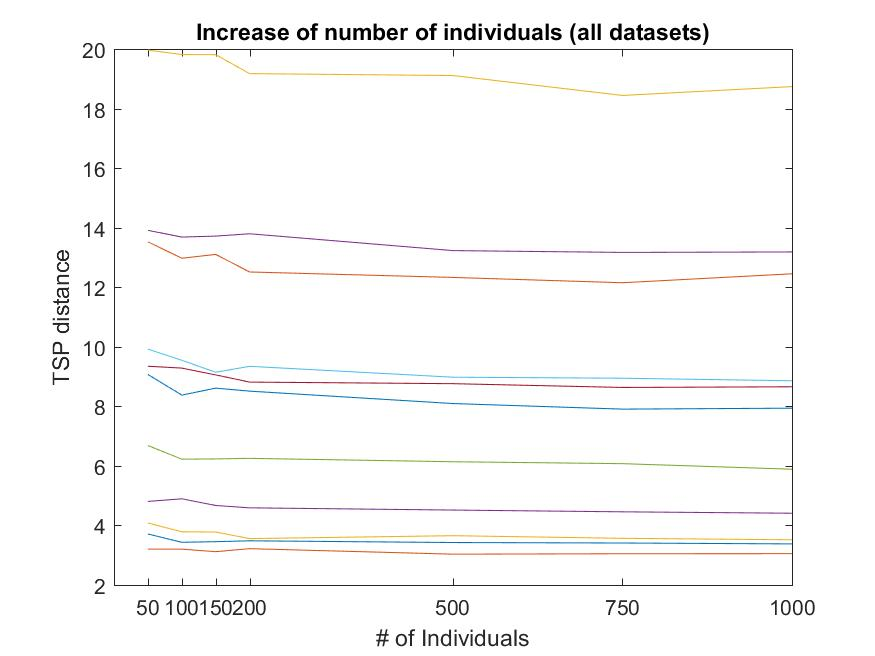
\includegraphics[width=12cm]{img/xalt_edges/numberIndiv.jpg}
\end{center}
\subsubsection{Original-General-Generations}
\begin{center}
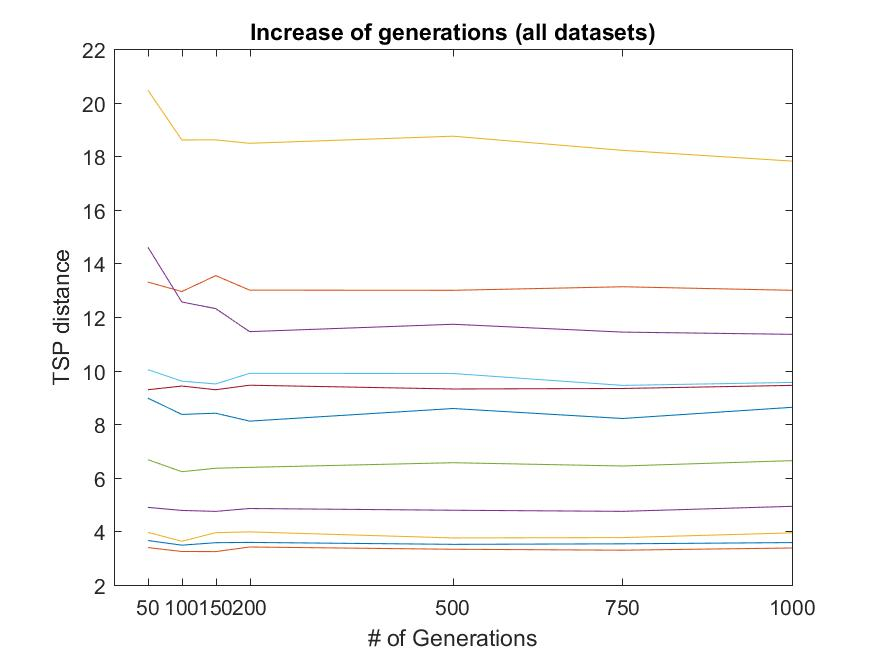
\includegraphics[width=12cm]{img/xalt_edges/numberGens.jpg}
\end{center}
\subsubsection{Original-General-Elitism}
\begin{center}
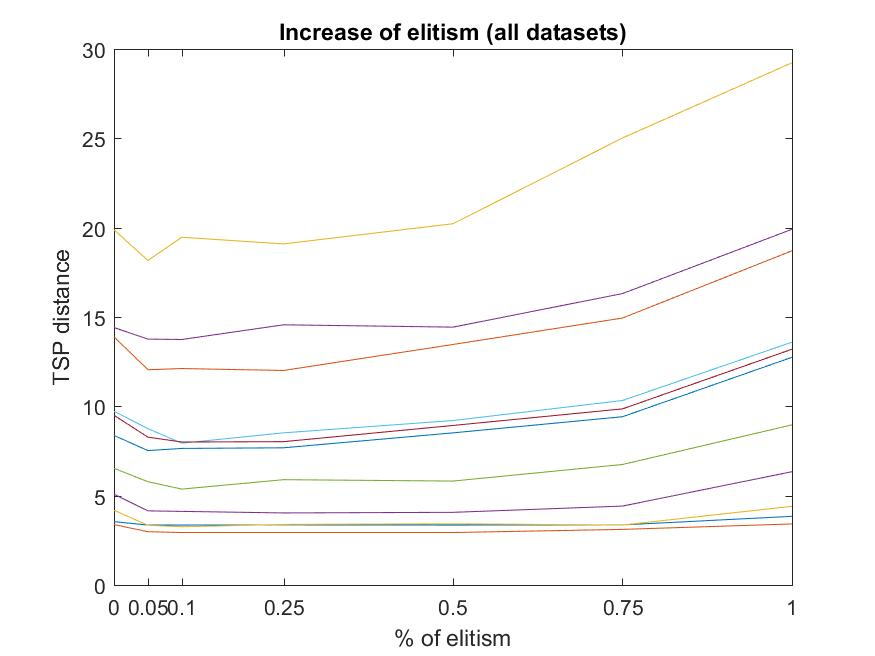
\includegraphics[width=12cm]{img/xalt_edges/elitism.jpg}
\end{center}
\subsubsection{Original-General-Crossover and mutation}
\begin{center}
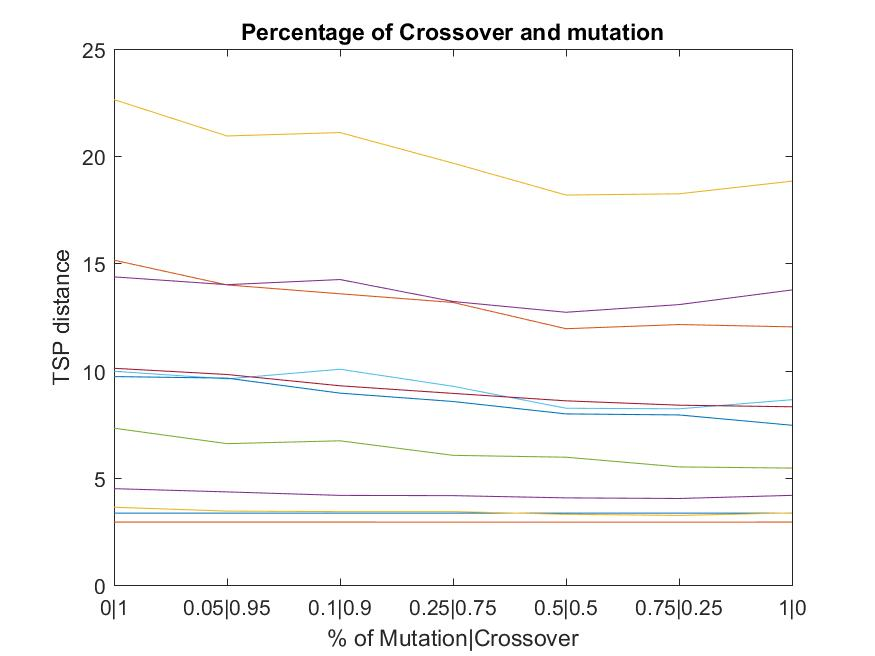
\includegraphics[width=12cm]{img/xalt_edges/crossMut.jpg}
\end{center}
\subsubsection{Modified-General-Individuals}
\begin{center}
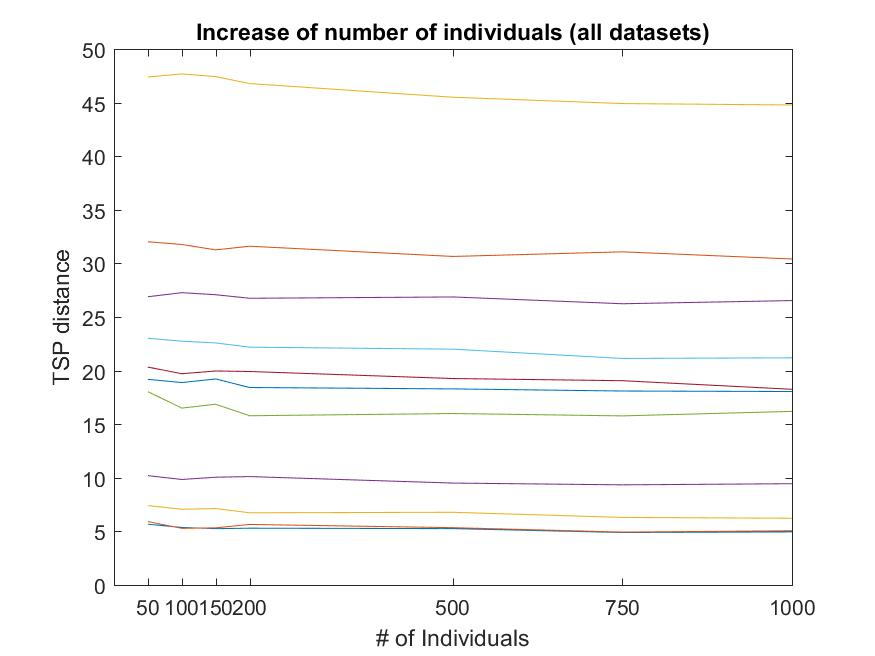
\includegraphics[width=12cm]{img/order_crossover/numberIndiv.jpg}
\end{center}
\subsubsection{Modified-General-Generations}
\begin{center}
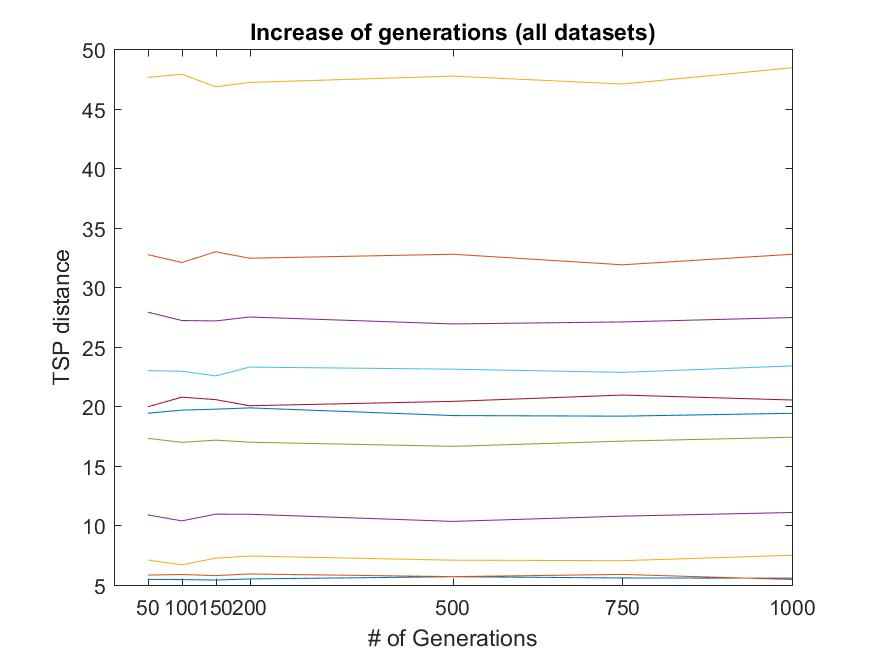
\includegraphics[width=12cm]{img/order_crossover/numberGens.jpg}
\end{center}
\subsubsection{Modified-General-Elitism}
\begin{center}
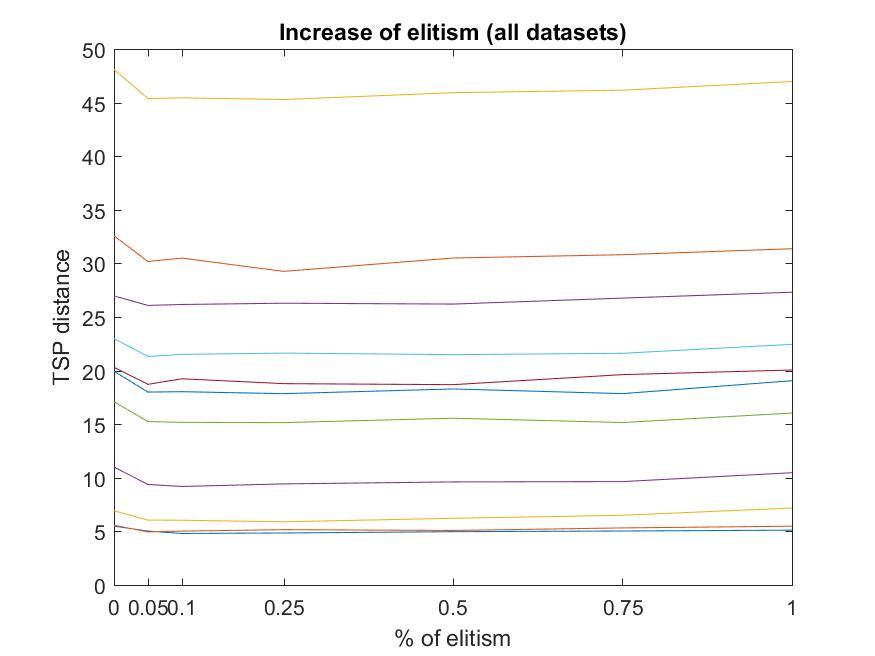
\includegraphics[width=12cm]{img/order_crossover/elitism.jpg}
\end{center}
\subsubsection{Modified-General-Crossover and mutation}
\begin{center}
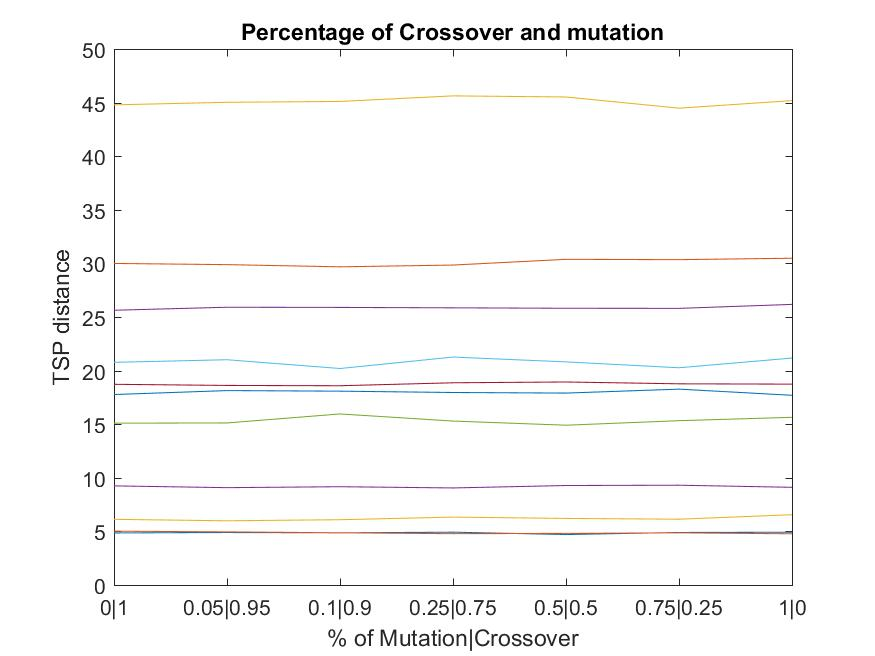
\includegraphics[width=12cm]{img/order_crossover/crossMut.jpg}
\end{center}








% End of function

